\section{Introduction}

Mass spectrometry (MS) is an important tool used to identify unknown molecular samples in a variety of applications, from characterization of organic synthesis products, to pharmacokinetic studies \cite{massspec_pharmakinetics}, to forensic studies \cite{Zhou2017LatentFingerprints}, to analyzing gaseous samples on remote satellites \cite{Petrie_ions_in_space}.

In electron-ionization mass spectrometry (EI-MS), molecular samples are ionized by an electron beam and broken into fragments. The resultant ions are separated by an electric field until they reach a detector. The mass spectrum is a distribution of the frequency or intensity of each type of ion, ordered by mass-to-charge (\textit{m/z}) ratio.

A popular method for identifying a sample from its mass spectrum is to look up the sample's spectrum in a \textit{reference library}. Here, a similarity function is used to measure the similarity between the query spectrum from the sample and each spectrum in the library. If the measurement noise when obtaining the query spectrum is reasonable, then the library spectrum with the highest similarity will have the identity of the sample.\cite{stein1995ChemicalSubstructureIdentification,stein1994optimization} A schematic of this process is shown in Figure~\ref{fig:library_matching}a.

This library matching approach is very popular, but it suffers from a \textit{coverage problem}: if the sample consists of a molecule that is not in the library, then correct identification is impossible. This is an issue in practice, since existing mass spectral reference libraries, such as the NIST/NIH/EPA MS database~\cite{2017nist}, Wiley Registry of Mass Spectral Data~\cite{mclafferty2016wiley}, and MassBank~\cite{horai2010massbank} only contain hundreds of thousands of reference spectra. The coverage problem could be reduced by recording spectra for additional molecules, but this is time consuming and expensive. For example, NIST releases updates to its library every 3 years, containing roughly 20,000 new spectra. Additionally, mass spectra of new molecules are only added to the library if the molecule is of common interest; molecules for newly synthesized compounds are typically not incorporated~ \cite{2017nist,stein2012MassLibReview}.

An alternative solution is to use \textit{de novo} methods that input a spectrum and directly generate a molecule, without using a fixed list of molecules (Section~\ref{sec:related-work}). However, these approaches currently have low-accuracy and are difficult for practitioners to incorporate into their existing work-flows.

Another method for alleviating the coverage problem is to augment existing libraries with synthetic spectra that are generated by a model. Thus far, this approach has not been practical, as existing spectrum prediction methods are very computationally expensive. These prediction models use quantum mechanics calculations ~\cite{bauer2016compute,grimme2013towards,Guerra_BEB_model} or machine learning~\cite{allen2016computational} to estimate the probability of each bond breaking under ionization, and thus the frequency of each ion fragment. Since these methods must either compute molecular orbital energies with high accuracy using expensive calculations, or else stochastically simulate the fragmentation of the molecule, the time needed for each model to make a prediction scales with the size of the molecule, taking up to 10 minutes for large molecules \cite{bauer2016compute,allen2016computational}.

In response, we present Neural Electron Ionization Mass Spectrometry (NEIMS), a neural network that predicts the electron-ionization mass spectrum for a given small molecule. Since our model directly predicts spectra, instead of bond breaking probabilities, it is dramatically faster than previously reported methods, making it possible to generate predictions for thousands of possible candidates in seconds. Furthermore, the approach does not rely on specific details of EI, and thus our model could be easily retrained to predict mass spectra for other ionization methods.

We test the performance of our model by predicting mass spectra for small molecules from the NIST 2017 Mass Spectral Library. We find that the predictive capability of our model is similar to previously reported machine learning models, but requires much less time to make predictions. Additionally, we report the similarity of the spectra predicted by NEIMS. The code repository for NEIMS is publicly available at github.com/brain-research/deep-molecular-massspec.

\section{Related Work}
\label{sec:related-work}
Several algorithms have been developed previously for either predicting spectra or for predicting the molecule's identity given the spectrum. We review some of these techniques here.

%\begin{itemize}
\textbf{DENDRAL} One of the earliest efforts in artificial intelligence was a model used to identify molecules from their mass spectrum. Heuristic DENDRAL (Dentritic Algorithm) was a collaboration between chemists and computer scientists at Stanford in the 1960s~\cite{buchanan1981dendral}. This algorithm used expert rules from chemistry to help identify patterns in the spectra and suggest possible identities for the molecule. A few years later, Meta DENDRAL was introduced to learn the expert rules that originally been given to Heuristic DENDRAL~\cite{lindsay1993dendral}.

\textbf{De Novo Identification Methods} Several models have been reported to predict identities of samples directly from the spectrum. Many have been developed for tandem mass spectrometry, where the task is to predict the original peptide sequences from digested fragments given the mass spectrum~\cite{Eng1994sequest}. Some of these methods use machine learning to achieve this task~\cite{Tran8247deepnovo, Schoenholtz2018supervision}. One work even uses machine learning models to identify personal characteristics by analyzing electrospray-ionization mass spectra of samples collected from human fingerprints~\cite{Zhou2017LatentFingerprints}.

While this approach is common for prediction of peptide sequences, it is uncommon for prediction of molecules from spectra. Several previously published models have used neural network models to predict molecule subgroups from spectra, or the class of the molecule~\cite{curry1990msnet,spec2smiles}. One recent work attempts to employ a LSTM sequence-to-sequence model to predict the molecule directly from its mass spectrum, using the Simplified Molecular Input Line Entry Specification (SMILES) to output the molecule~\cite{spec2smiles}. Because of the difficulty of constructing syntactically correct SMILES, this approach was not able to successfully reconstruct the entire SMILES string for any of the input spectra.

In this work, we focus on the prediction of spectra from molecules, such that these predicted spectra can be used to improve the coverage of library-matching-based identification. The advantage of this approach over de novo approaches is that new libraries of synthetic spectra can be easily incorporated into the existing mass spectrometry software used by practitioners.
\textbf{Quantum Mechanics Spectral Prediction Methods}
he first prediction methods for EI-MS spectrum used quantum mechanical simulation techniques to predict fragmentation events. There are three methods of predicting the mass spectrum using first principles~\cite{bauer2016compute}.
The first is to use quasi-equilibrium theory, also known as Rice-Ramsberger-Kassel-Marcus theory, to estimate the rate constants for ionization reaction~\cite{lorquet1994whither, lorquet2000landmarks, rosenstock1952absolute}.
The second is to estimate the bond order energies within a molecule, and estimate where a molecule may fragment. A related method to this second method is to calculate the cross-section of molecular orbitals upon electron impact to predict the molecule's ionization behavior~\cite{irikura2017ab, Guerra_BEB_model}.
The third method uses Born-Oppenheimer Molecular Dynamics. Quantum Chemistry Electron-Ionization Mass Spectrometry (QCEIMS) is a particularly recent example of the ab initio molecular dynamics method~\cite{grimme2013towards,Asgeirsson_QCEIMS,bauer2016compute}.
The trajectories resulting from this simulation are then analyzed for the presence of ionic fragments. The distribution of the ion fragments aggregated from all the simulations is then renormalized to generate a calculated EI-MS spectrum.
Each of these methods requires at least 1000 seconds per molecule \cite{allen2016computational}, and may even take days or weeks for molecules of 50 atoms. While these methods may be fast for methods involving density functional theory, they do not have the speed needed to rapidly generate a collection of spectra thousands of molecules. Furtermore, some of the basis sets used for the density functional theory might not support the presence of inorganic atoms.

\textbf{Machine Learning Spectral Prediction Methods} Allen et al.~\cite{allen2016computational} introduced Competitive Fragmentation Modelling-Electron Ioinization (CFM-EI) to predict EI-MS spectra. This probabilistic model predicts the probability of breaking molecular bonds under electron ionization, and also predicts the charged fragment that is likely to form. In order to generate the spectra, it is necessary to run a stochastic simulation to determine the frequency of each molecular fragment.
In Section~\ref{sec:NIST14-results}, we directly compare this method with our proposed model.






\begin{figure}[t]
    \centering
    \begin{subfigure}{0.9\textwidth}
        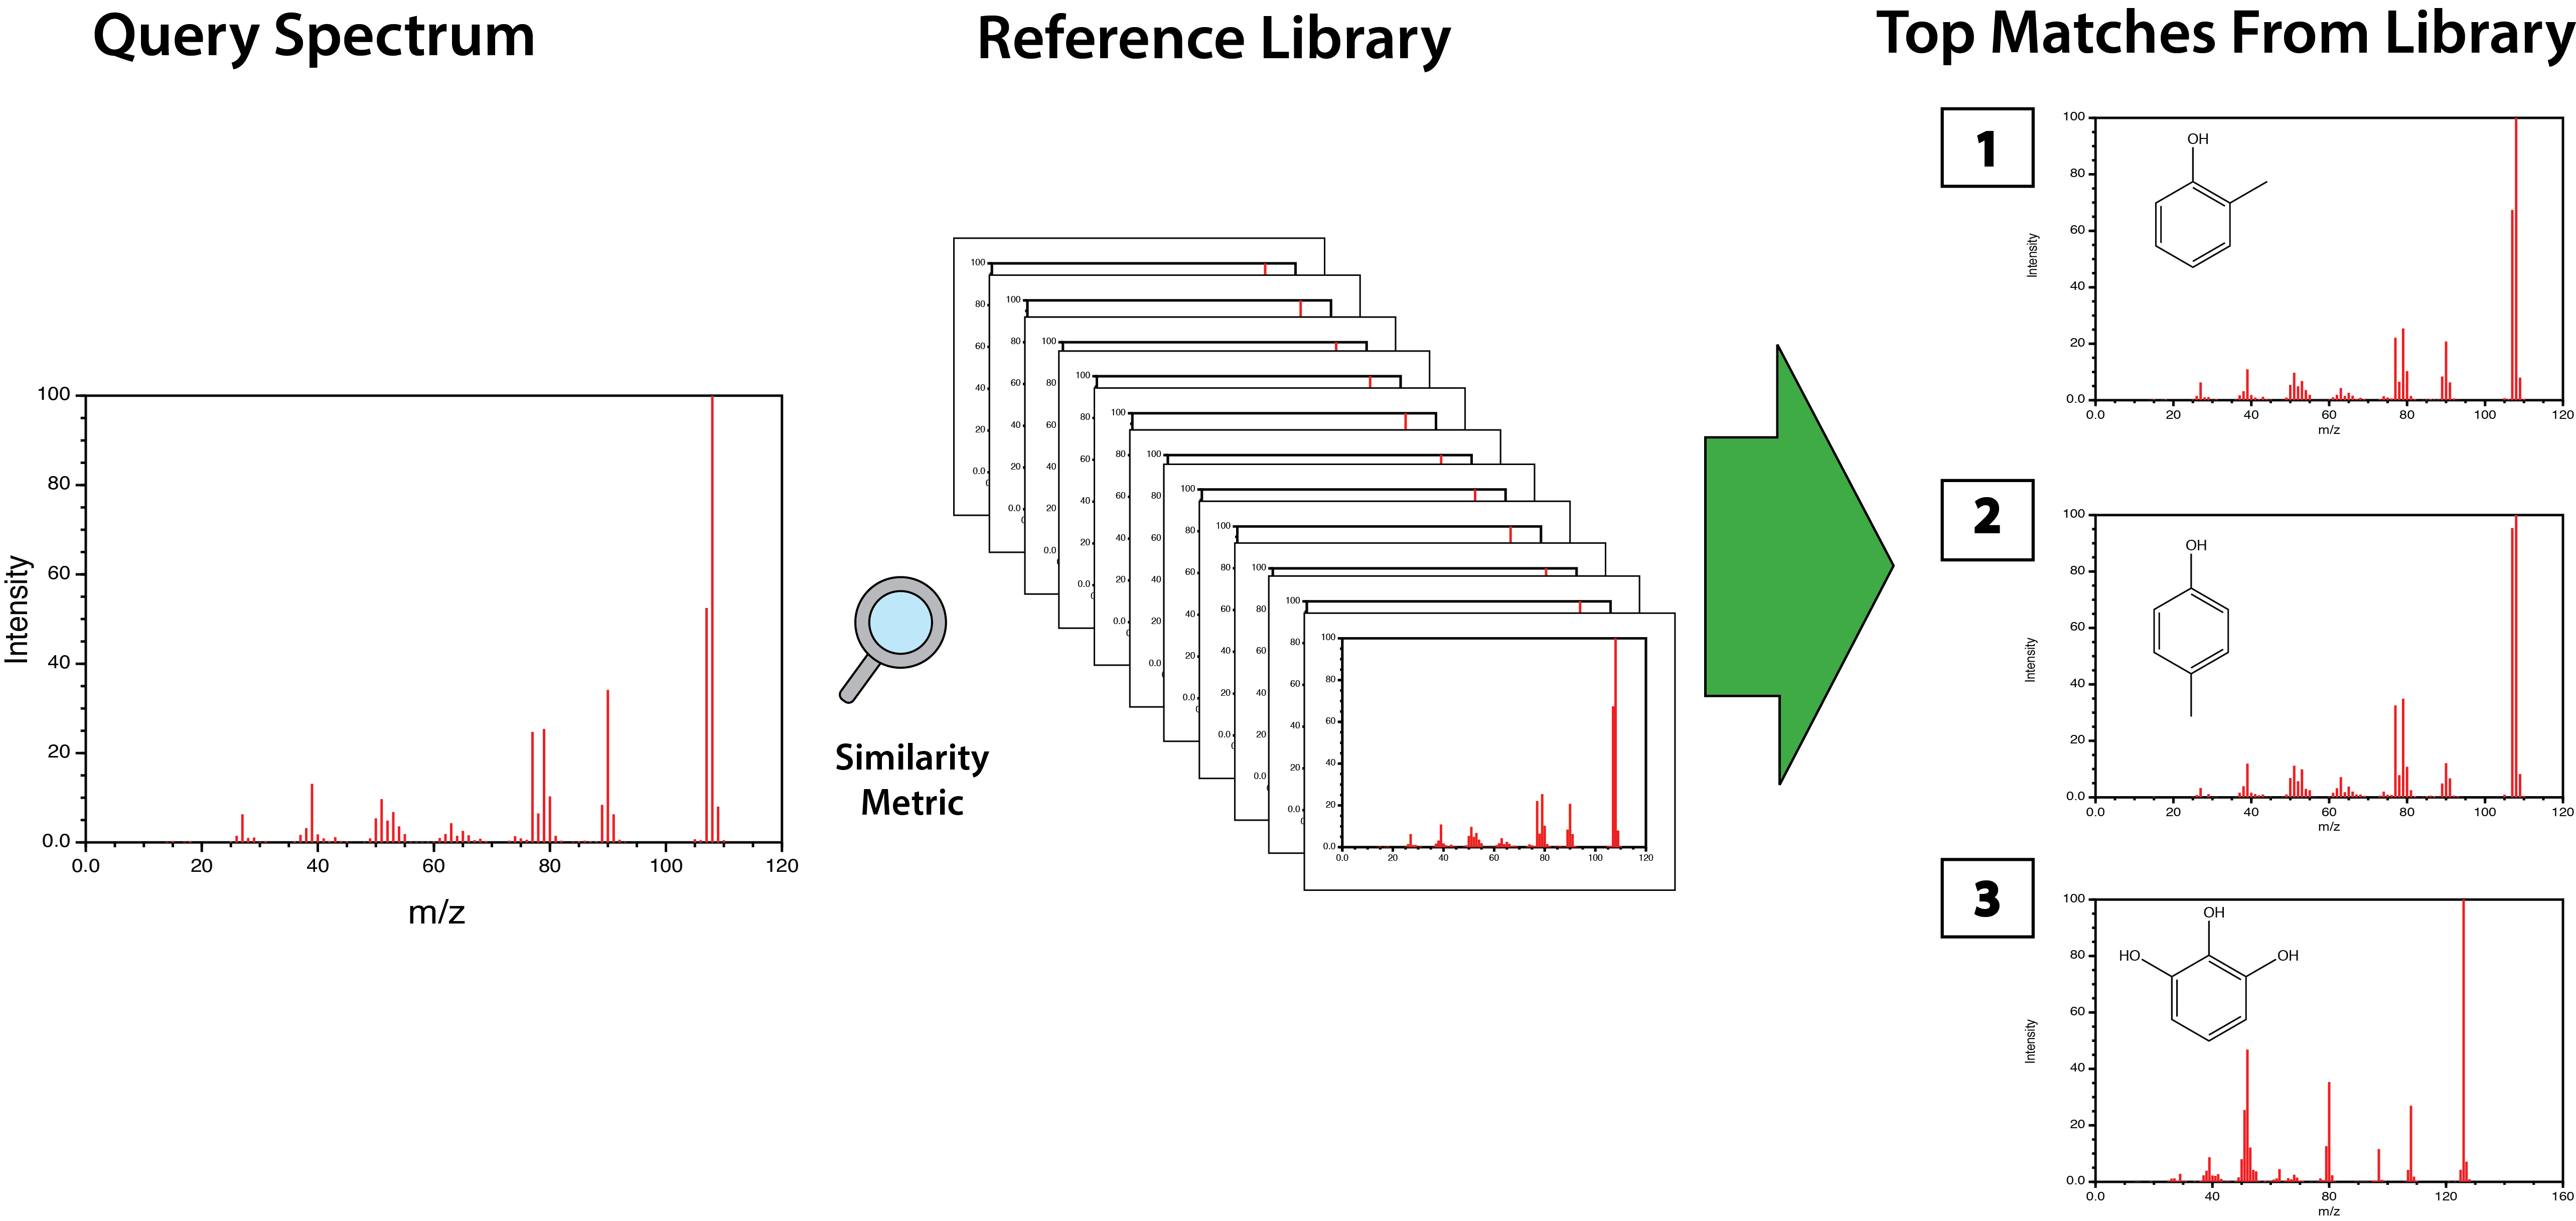
\includegraphics[width=\textwidth]{./lib_match_baseline.png}
        \caption{}
    \end{subfigure}
    \begin{subfigure}{0.9\textwidth}
        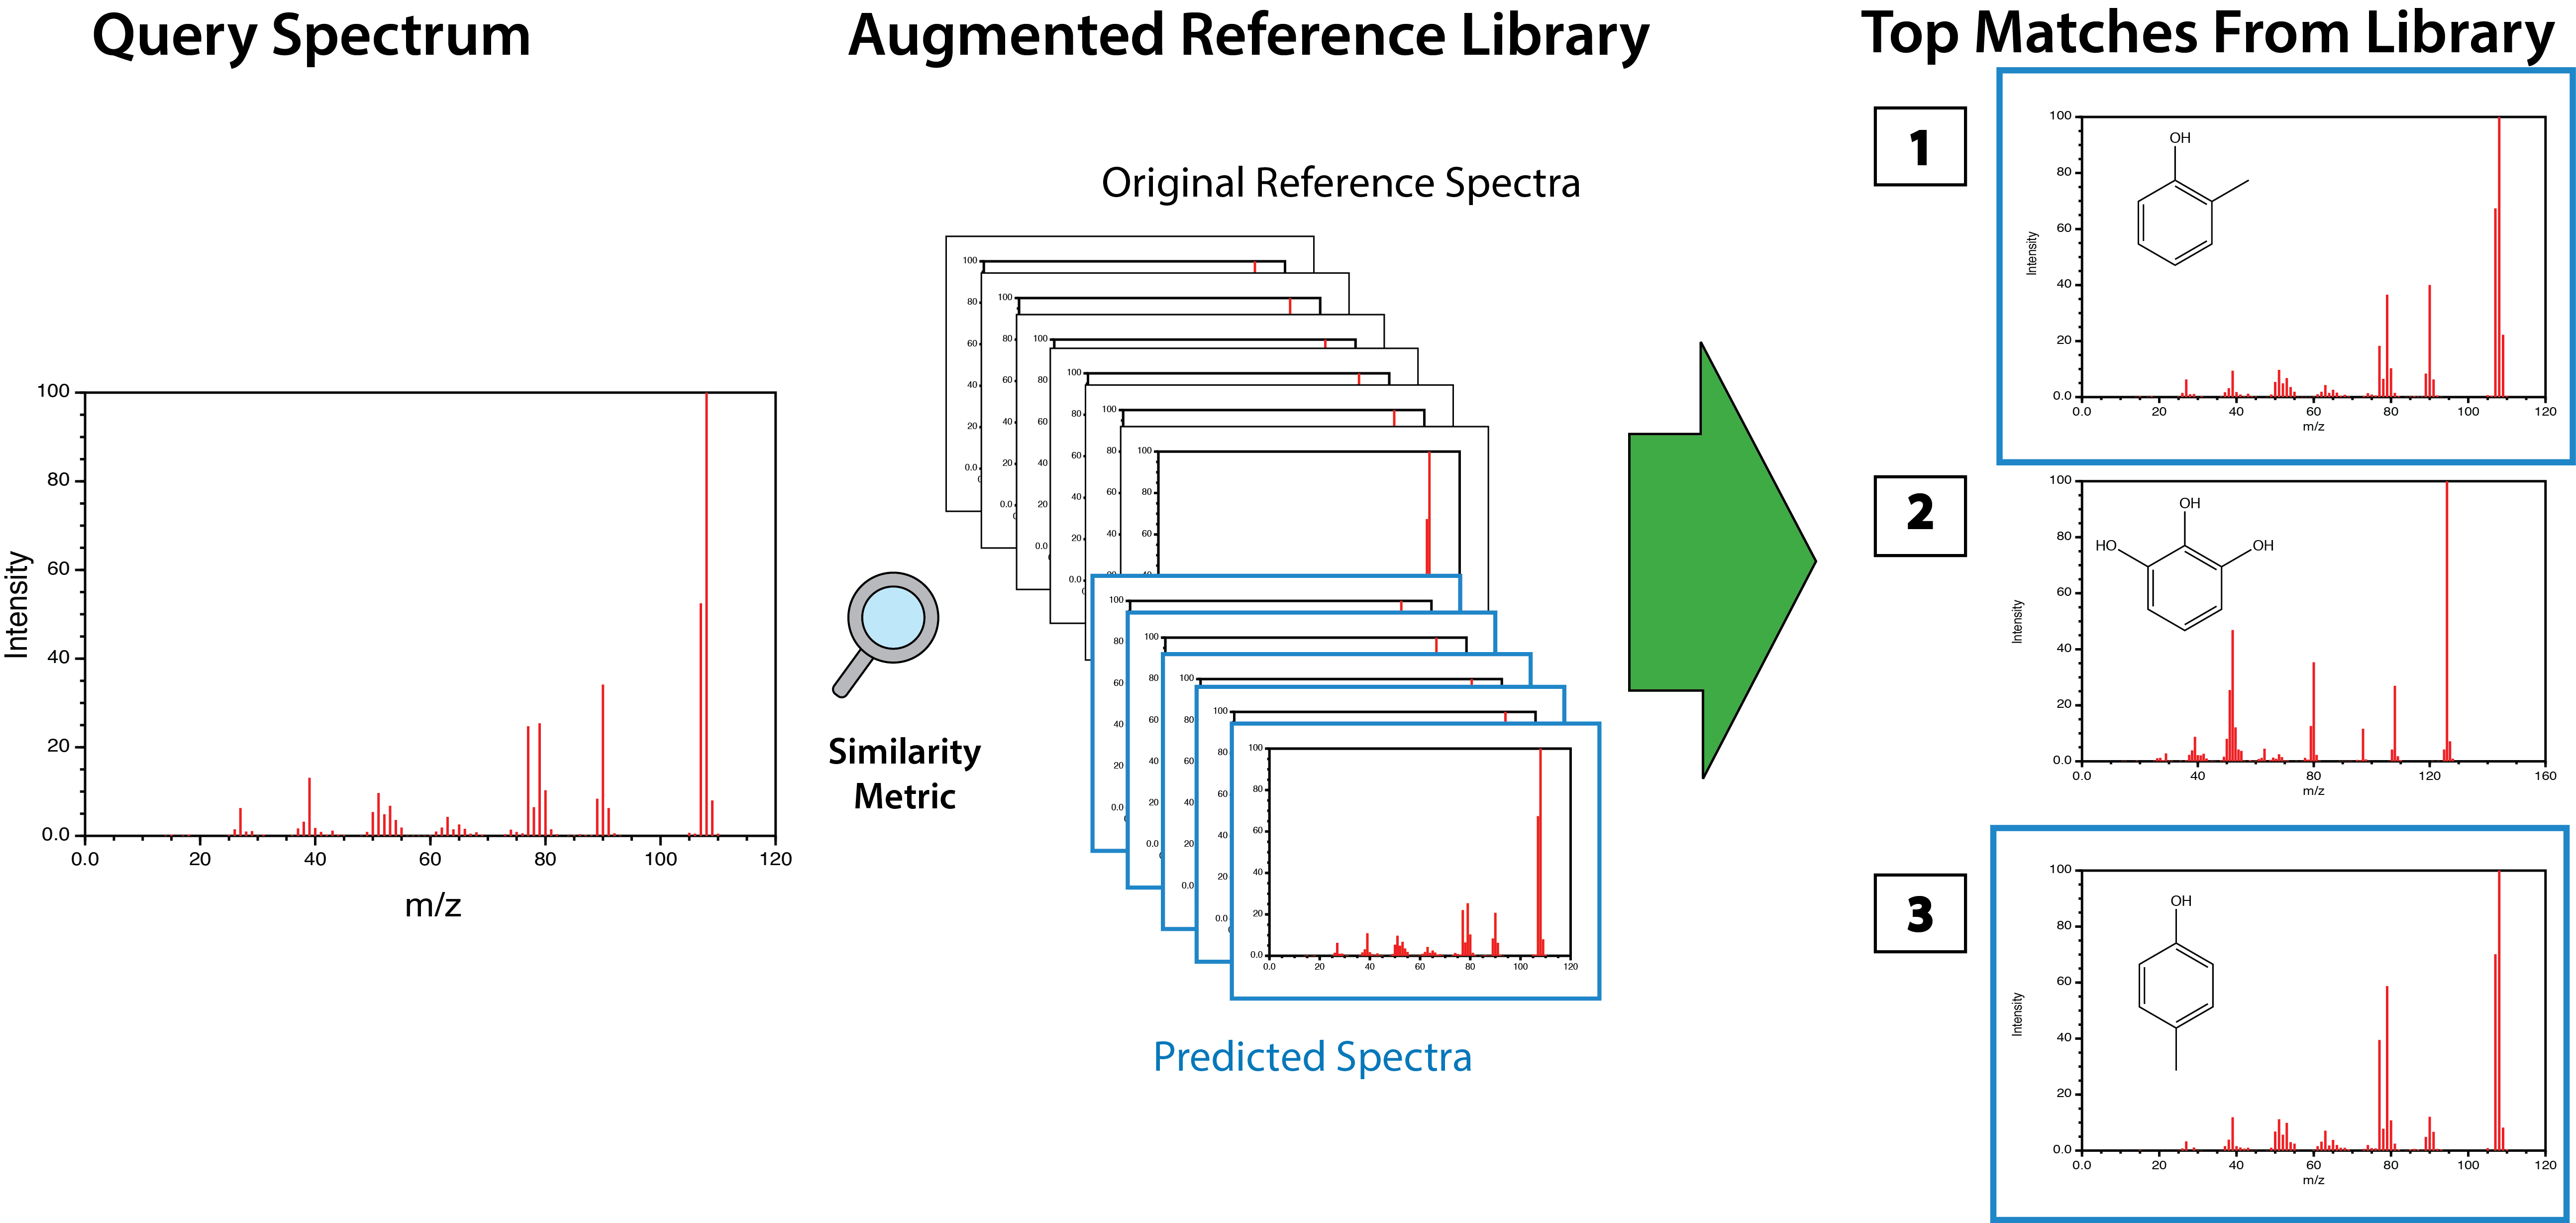
\includegraphics[width=\textwidth]{./lib_match_predicted.png}
        \caption{}
    \end{subfigure}
    \caption[Library Matching Task]{Library Matching Task.~(a) A depiction of how query spectra are matched to a collection of reference spectra as performed by mass spectrometry software. (b) Query spectra are compared against a library comprised of spectra from the NIST 2017 main library and spectra predicted by our model (outlined in blue).  Spectral Images adapted from NIST Webbook~\cite{NIST_WebBook}.}
    \label{fig:library_matching}
\end{figure}

\section{Methods}


Our goal is to design a model that will accurately predict the EI-MS spectrum for any molecule. This will be used to produce an augmented reference library containing both predicted spectra and experimentally-measured spectra.  This task is outlined in Figure \ref{fig:library_matching}b.

We first discuss how similarity metrics for spectra in Section \ref{sec:similarity_discussion}. Next, we describe our method for spectra prediction in Sections \ref{sec:ms_spectral_prediction} and \ref{sec:ms_physical_phenomena}. We then explain how we evaluate our model's impact on the library matching task more thoroughly in Section \ref{sec:library_matching_description}.


\subsection{Similarity Metrics for Mass Spectra}\label{sec:similarity_discussion}

The ability to a match a query spectrum from a sample to the correct spectrum in the library depends on the choice of similarity metric between spectra~\cite{mclafferty1974probability,stein1994optimization}.
A weighted cosine similarity is commonly used by mass spectrometry software. The exact form of the cosine similarity is given below~\cite{stein1994optimization}:

\begin{equation}\label{eq:stein-similarity}
\text{Similarity}(\boldsymbol{I}_q, \boldsymbol{I}_l) = \frac{\sum_{k=1}^{M_{max}} m_{k} I_{qk}^{0.5} \cdot m_{k} I_{lk}^{0.5}}{\left\lVert\sum_{k=1}^{M_q} (m_{k} I_{qk}^{0.5})^2\right\rVert \left\lVert\sum_{k=1}^{M_l} (m_{k} I_{lk}^{0.5})^2\right\rVert}.
\end{equation}
Here, {$\boldsymbol{I}_q$} and {$\boldsymbol{I}_l$} are vectors of \textit{m/z} intensities representing the query spectrum and the library spectrum respectively, $m_k$ and $I_k$ are the mass-to-charge ratio and intensity found at $m/z = k$, $M_l$ and $M_q$ are the largest indices of $\boldsymbol{I}_q$ and $\boldsymbol{I}_l$ with non-zero values,and $M_{max}$ is the larger of $M_l$ and $M_q$. The motivation for the weighting by $m/z$ is because the peaks in mass spectra corresponding to larger fragments are more characteristic and useful in practice for identifying the true molecule.

Other similarity metrics besides cosine distance similarities are also employed. For example, one other similarity method involves estimating the relative importance of one peak given the other peaks~\cite{mclafferty1974probability}. Other methods uses a Euclidian difference between peaks, or use a variation of the Hamming distance~\cite{stein1994optimization,hertz1971identification}. Another similarity metric accounts for neutral losses, or the intensity peaks corresponding to the loss of small, neutral fragments from the original molecular ion~\cite{moorthy2017combining}. It is also possible to use the same form of the similarity function as in \eqref{eq:stein-similarity}, but with different weighting given to the intensity or the masses~\cite{stein1994optimization}. In principle, machine learning could be also used to learn a parameterized similarity metric that yields improved library matching performance. However, this custom metric would be difficult to deploy, since it would require changing the software used by practitioners.

We develop our model with the assumption that Eq.~\eqref{eq:stein-similarity} will be used for the similarity metric in downstream library matching software that consumes an augmented library.

\subsection{Spectral Prediction}\label{sec:ms_spectral_prediction}

We treat the prediction of mass spectrometry spectra as a multi-dimensional regression task. The output of our model is a vector that represents the intensity at every integral \textit{m/z} bin. We use this discretization granularity for \textit{m/z} because it is what is provided in the NIST datasets we use for training our model.

In the NEIMS model (Figure~\ref{fig:model_prediction}), we first map molecules to additive Extended Circular Fingerprints (ECFPs)~\cite{rdkit}.
These fingerprints are similar to their binary counterparts~\cite{Rogers_2010_ECFP} in that they record molecular subgraphs made up from local neighborhoods around each atom node in the molecule, but differ in that they count the occurrences for each subgroup. This information is then hashed into a vector representation. The difference is that additive fingerprints record the frequency that each bit is set, rather than just the presence. The RDKit Cheminformatics package~\cite{rdkit} was used to generate the fingerprints.
These features are then passed into a multi-layer perceptron neural network (MLP).
To account for some of the physical phenomena of ionization, we make some application-specific adjustments to the prediction from the MLP, described in Section~\ref{sec:ms_physical_phenomena}.

In Section~\ref{sec:library-matching-results} we compare the performance of NEIMS to that of a simple linear regression (LR) model. Here, we apply a linear transformation to the ECFP features.

To train the model, we use a modified mean-squared-error loss function. This loss function, shown below, follows the same weighting pattern as in Eq.~\ref{eq:stein-similarity}:

\begin{equation}\label{eq:training_loss}
    L(\boldsymbol{I}, \hat{\boldsymbol{I}}) = \sum_{k=1}^{M(x)} \left(\frac{m_k I_k^{0.5}}{\left\lVert\sum_{k=1}^{M} (m_{k} I_{k}^{0.5})^2\right\rVert} - \frac{m_k \hat{I_k}^{0.5}}{\left\lVert\sum_{k=1}^{M} (m_{k} \hat{I}_{k}^{0.5})^2\right\rVert}\right)^2
\end{equation}

where $I$ is the ground truth spectrum, $\hat{I}$ is the predicted spectrum, and $M(x)$ is the mass of the input molecule.
We used stochastic gradient descent to optimize the parameters of the MLP with the Adam optimizer~\cite{Kingma_adam_optimizer}. We use Tensorflow~\cite{Tensorflow-2016} to construct and train the model.

\subsection{Adjustments for Physical Phenomena}\label{sec:ms_physical_phenomena}

In practice, we have found that the conventional MLP described in the previous section struggles to accurately predict the right-hand side of spectra (Figure~\ref{fig:MLP_improvement_spectra}a). Errors in this region, which correspond to large $m/z$, are particularly damaging for library matching with the weighting in~\eqref{eq:stein-similarity}.

This section introduces a revised neural network architecture (Figure~\ref{fig:model_prediction}) designed to better model the underlying fragmentation process that occurs in mass spectrometry. We have found that it improves prediction in the high mass region of the spectrum (Figure~\ref{fig:MLP_improvement_spectra}b), which yields improvements in library matching (Section~\ref{sec:library-matching-results}).

As is standard for MLPs used for regression, the predictions of the above MLP model on an input molecule $x$ are an affine transformation of a set of features $f(x)$, which are computed by all but the final layer of the network. For reasons that will become apparent, we refer to the above MLP as performing \textit{forward} prediction. At bin $m/z = i$, we have the following predicted intensity:
\begin{equation}
p^f_i(x) = w^{f\top}_i f(x) + b^f_i, \label{eq:pred-i}
\end{equation}
where $w^f_i$ and $b^f_i$ are the model's weights and biases for forward prediction at bin $i$.

The input ECFP features, from which $f(x)$ is computed, capture local structures in the molecule, so generally $f(x)$ will be more accurate in capturing the presence of small substructures of molecule $x$. Often, there is a direct correspondence between the presence of such substructures and spectral peaks with small $m/z$. For example, in Figure \ref{fig:MLP_improvement_spectra}a a peak occurs at $m/z = 35$, due to the presence of chlorine. Therefore an accurate forward prediction model will have a learned weight $w_{35}$ that will output a high intensity at $i = 35$ if there is evidence in $f(x)$ for the presence of chlorine.

\begin{figure}[t]
    \centering
    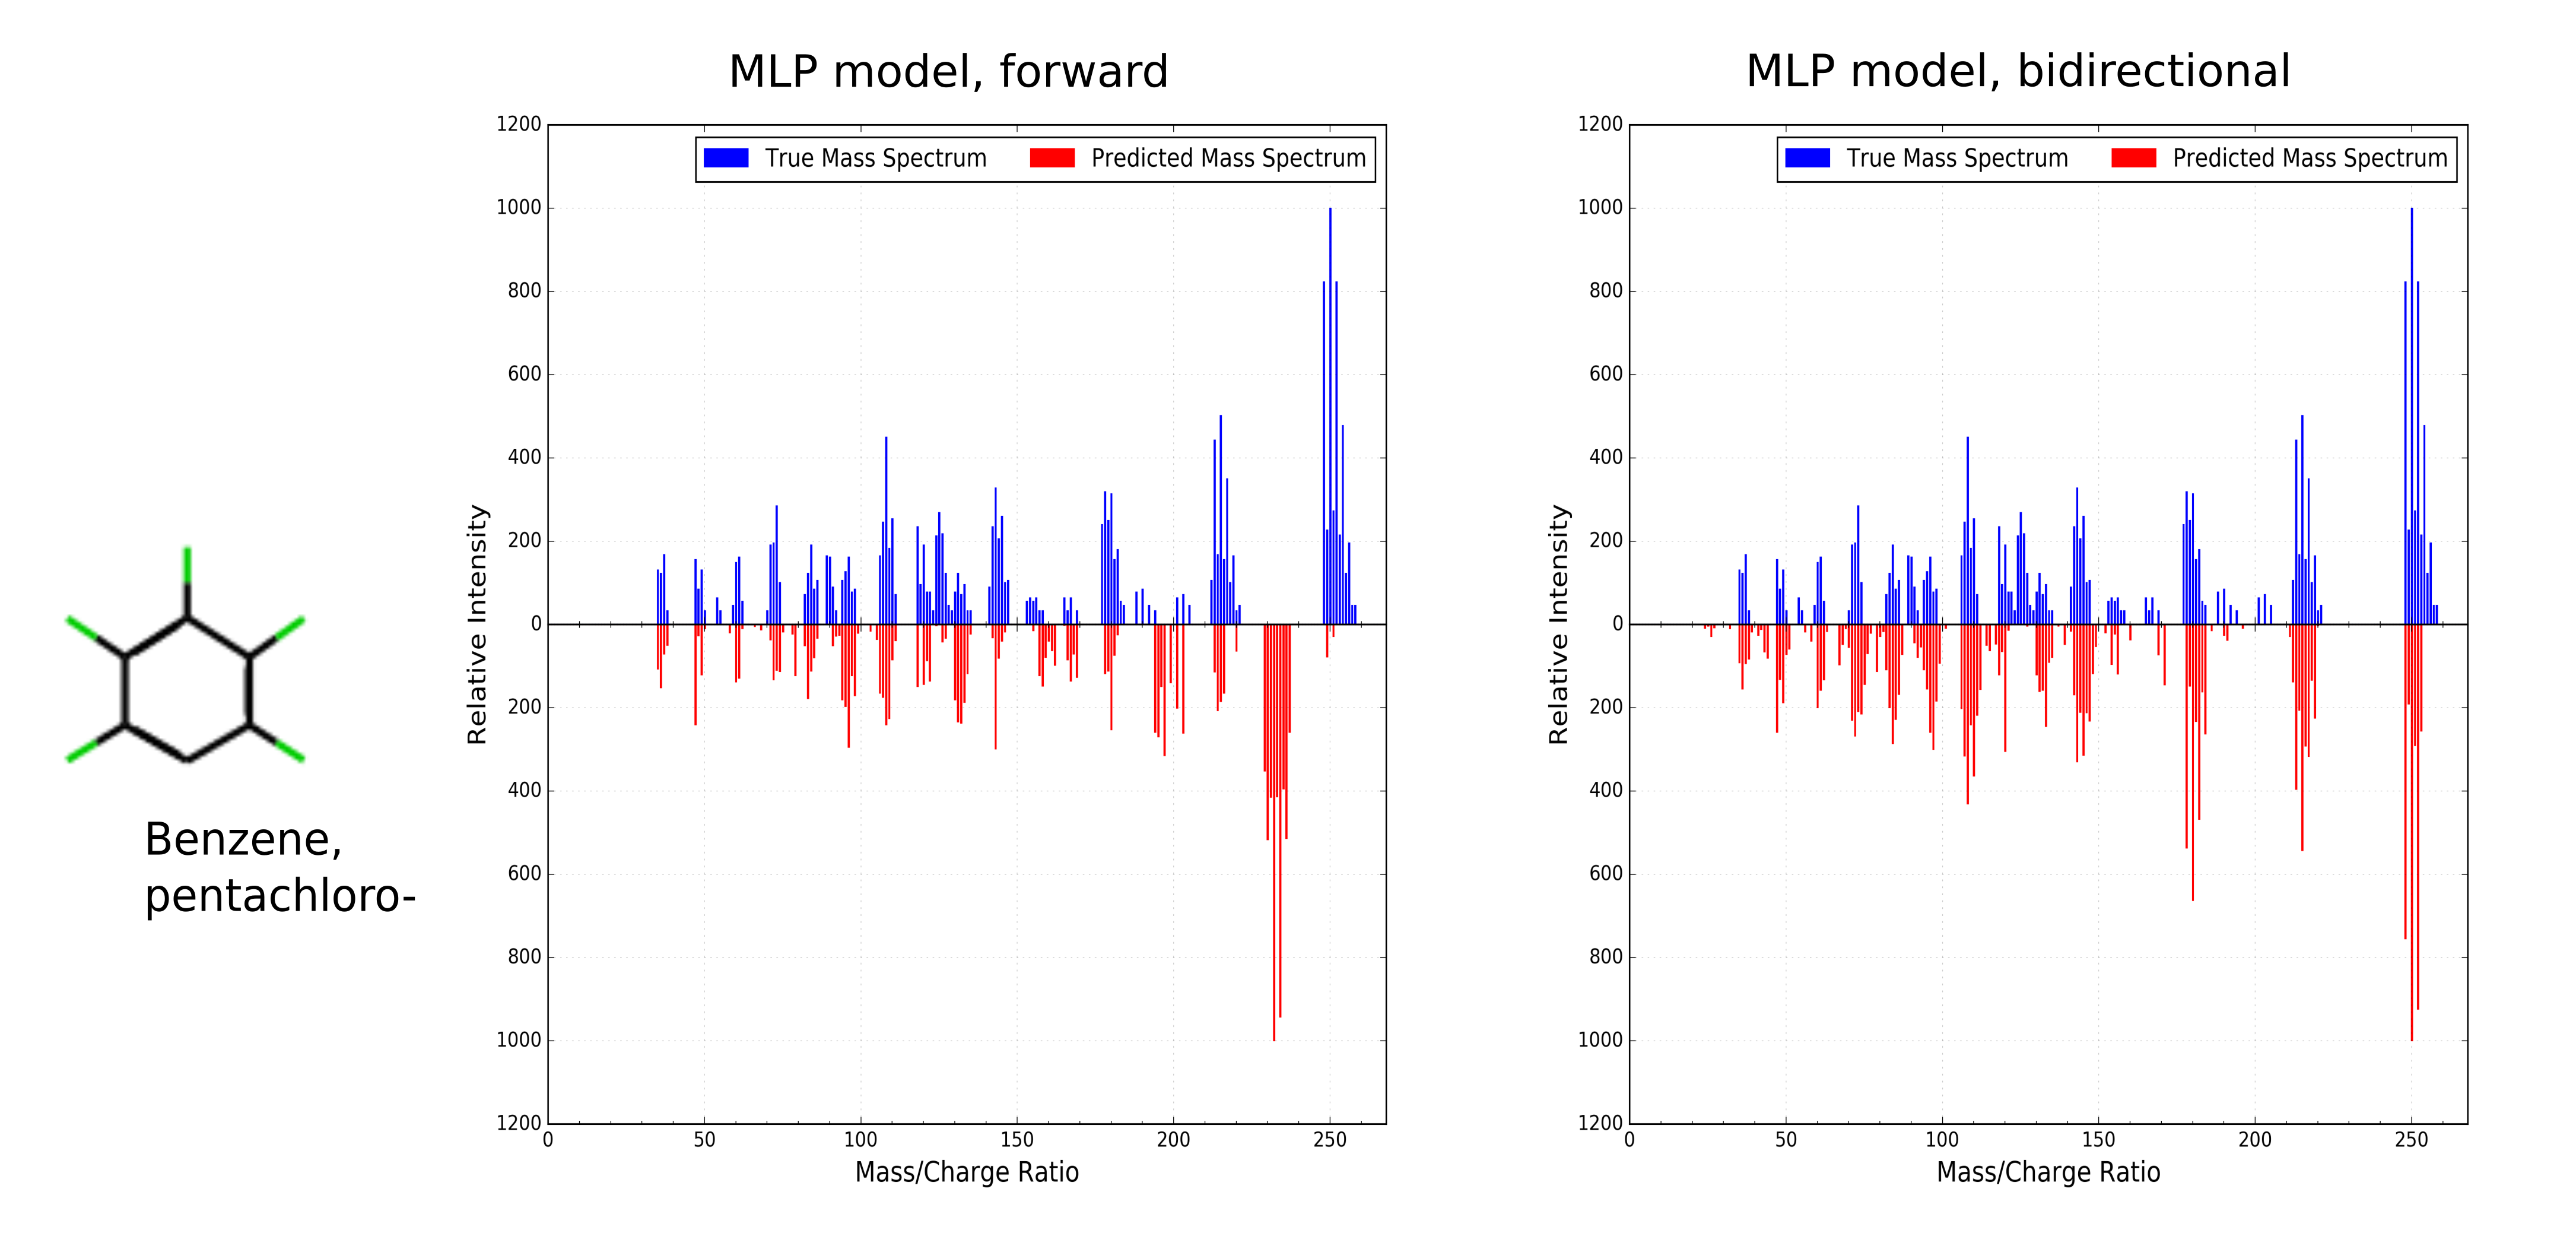
\includegraphics[width=0.9\linewidth]{./CEOCDNVZRAIOQZ-UHFFFAOYSA-N_mlp_model_spectra.png}
        \caption[Sample Spectra Prediction]{Spectral Prediction with MLP forward Model (a) and MLP bidirectional Model (b). For both spectra plots, the true spectrum is shown in blue on top, while the predicted spectrum is shown inverted in red. ~Note that the spectrum predicted by the bidirectional model shows fewer stray peaks than the forward model, particularly for larger \textit{m/z} values. These peaks are much easier to predict with the reverse prediction mode.}
    \label{fig:MLP_improvement_spectra}
\end{figure}


On the other hand, forward prediction often struggles to accurately predict intensities for large fragments that are the result of neutral losses~\cite{stein1995ChemicalSubstructureIdentification}. One reason for this is that the composition of large fragments is not captured well by the ECFP representation. Another reason is that information learned about the cleavage of a small group does not transfer well across molecules of different masses. For pentachlorobenzene, which has a molecular mass of 250 Da, the fragment that results from the loss of a neutral chlorine atom results in a peak at 215 Da. Meanwhile, for chlorobenzene, which has a mass of 112 Da, the fragment resulting from a loss of a chlorine atom would have a peak at 77 Da. Despite the clear relationship between these intensity peaks, the forward model is not parameterized to capture this pattern.

In response, following the physical phenomenon that created the fragments, we define larger ion peaks as a function of the residual groups that were broken off from the original molecule.
Referring to our previous example of pentachlorobenzene ($M(x) = 250$), we can parameterize the $m/z$ ratio of the fragment which lost a chlorine group as $m/z = 250 - 35 = 215$. The corresponding fragment in chlorobenzene would have a mass of $m/z = 215 - 35 =  77$. By defining the peaks in this way, it is possible for these predictions of spectral intensities to be linked by the prediction at index 35.
This leads to the indexing scheme of our \textit{reverse prediction} model:
\begin{equation}
p^r_{M(x) + \tau - i}(x) = w^{r\top}_i f(x) + b^r_i, \label{eq:pred-i-reverse}
\end{equation}
Here, $\tau > 0$ is a small shift that allows for peaks to occur at intensities greater than $M(x)$, due to isotopes. In practice, reverse prediction is implemented using a copy of the forward model, with separate sets of parameters for the final affine layer, but shared parameters for $f(x)$. The outputs of this model are post-processed on a per-molecule basis to obey the indexing in~\eqref{eq:pred-i-reverse}, which depends on each molecule's mass.

Both the forward and reverse predictions are combined to form a \textit{bidirectional} prediction. That is, the final prediction at index $i$ is a combination of both $p^f_i$ and $p^r_i$. In the case of pentachlorobenzene, the prediction of spectral intensity at $m/z = 215$ is a function of $p^f_{215}$ from the forward mode and $p^r_{35 + \tau}$ from the reverse mode. Instead of simply averaging the two prediction modes, we have found that small additional performance improvements can be obtained using a coordinate-wise \textit{gate}. Here, the output $p_i(x)$ at position $i$ is given by:
\begin{equation}\label{eq:sigmoid_gate}
p_i(x) = \sigma(\text{gate}_i) ~ p^f_i(x) + (1 - \sigma(\text{gate}_i)) ~ p^r_{i}(x),
\end{equation}
where $\text{gate}_i$ is an affine transformation of $f(x)$ and $\sigma(\cdot)$ is a sigmoid function. This approach echoes the formulation of the Hybrid Similarity Search designed by Moorthy et al., which accounts for peaks that are created by small fragment ions and those which are created by large fragments which have lost smaller groups~\cite{moorthy2017combining}.

Finally, for all models, we zero out predicted intensities at $m/z$ that are greater than $M(x) + \tau$.

By adding these features, we incorporate some of the physical phenomena that occur in mass spectrometry into our model while maintaining the overall simplicity of the MLP. In this way, we are able to predict the spectrum directly without resorting to sampling bond-breaking events within the molecule, which requires subsequent stochastic sampling to obtain a spectrum.

%In using the MLP architecture to model mass spectrometry fragmentation, our model is not directly a function of each bond in the molecule, allowing us to make quick calculations.
%We will examine the effects of adding these adjustments in Section \ref{sec:library-matching-results}.

\begin{figure}[t]
    \centering
    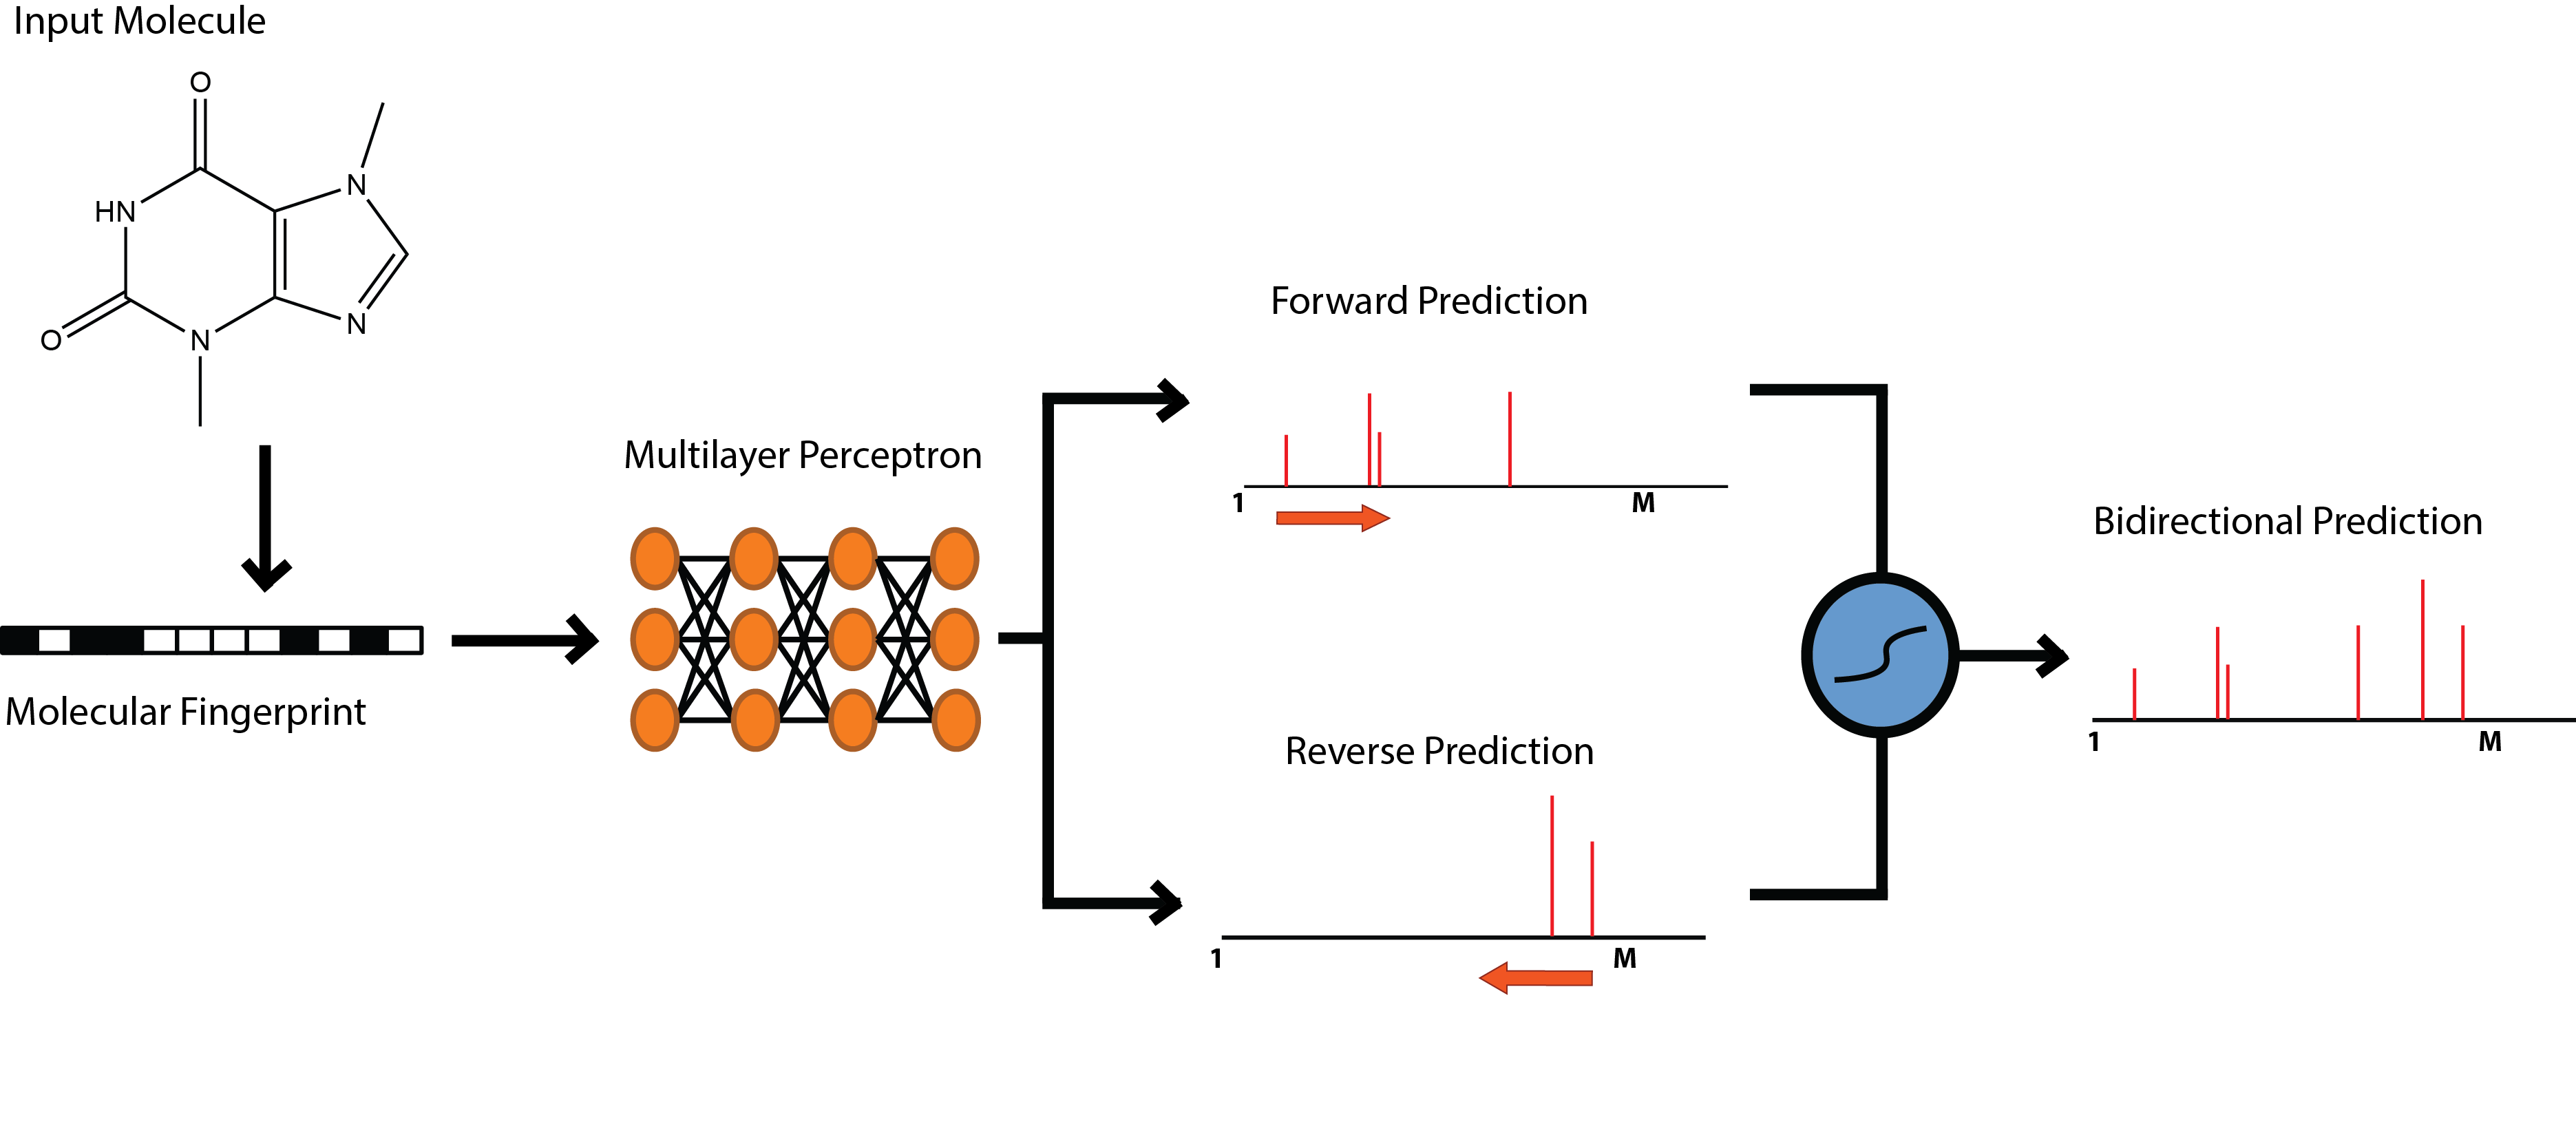
\includegraphics[width=0.9\linewidth]{./Model_prediction.png}
    \caption[Neural Electron Ionization MS Prediction Model]{Molecular representations are passed into a multilayer perceptron to generate an initial output. This output is used to make a forward prediction starting at $\textit{m/z}=0$ and $\textit{m/z}=M$ and in reverse starting from $\textit{m/z}=M$ and ending at $\textit{m/z}=0$. A sigmoid gating is applied to the inputs as shown in Eq. \ref{eq:sigmoid_gate}}
    \label{fig:model_prediction}
\end{figure}


\subsection{Library Matching Evaluation}\label{sec:library_matching_description}

We evaluate NEIMS using an \textit{augmented reference library} consisting of a combination of observed spectra and model-predicted spectra, with library matching performance computed with respect to a \textit{query set} of spectra. These are from the NIST 2017 replicates library, which is a collection of noisier spectra for molecules that are contained in the NIST main library. The inconsistencies in these spectra reflect experimental variation, and make an informative dataset to test our model's performance.

To construct the augmented reference library, we edit the NIST main library, removing spectra corresponding to the query set molecules and replacing them with the predictions from NEIMS.
We then perform library matching and calculate the similarity between each query spectrum and every spectrum from the augmented library. We record the rank of the correct spectrum, i.e. the rank of the predicted spectrum corresponding to the molecule which made the query spectrum. The similarity metric is Eq.~\eqref{eq:stein-similarity}.

For the purposes of tuning model hyperparameters, we chose to optimize recall@10, i.e. the percentage of our query set for which the correct spectra had a matching rank of less than or equal to 10 in the library matching task. Half of the replicates library was used for tuning hyperparameters, and the remaining half was used to evaluate test performance. All models were trained on the spectra prediction task for 100,000 training steps with a batch size of 100.

During the library match search, we have a \textit{mass filtering} option. This feature reduces the library size so it only includes spectra from molecular candidates that have a molecular mass that differ by a few Daltons from the mass of the query molecule.
If the EI-MS analysis is combined with mass spectrometry techniques using weak ionization methods, it is possible to determine the mass of molecule being analyzed. In the CFM-EI model, the molecular formula is used to filter the search library
~\cite{allen2016computational}. Using the molecular mass to filter the library allows more possible candidate spectra to be considered in the search than using a molecular formula filter.

\section{Results and Discussion}

To analyze the performance of the models, we trained with 240,942 spectra from the NIST 2017 Mass Spectral Main Library. These spectra were selected so that no molecules in the replicates library have spectra in the training set.

After hyperparameter tuning using Vizier~\cite{Google_Vizier}, we found that the optimal MLP architecture has seven layers of 2000 nodes, with residual network connections between the layers~\cite{he_resnet}, using ReLU activation and a dropout rate of 0.25.

\subsection{Library Matching Results}
\label{sec:library-matching-results}
\begin{figure}[t]
    \centering
    \begin{subfigure}[b]{0.52\linewidth}
        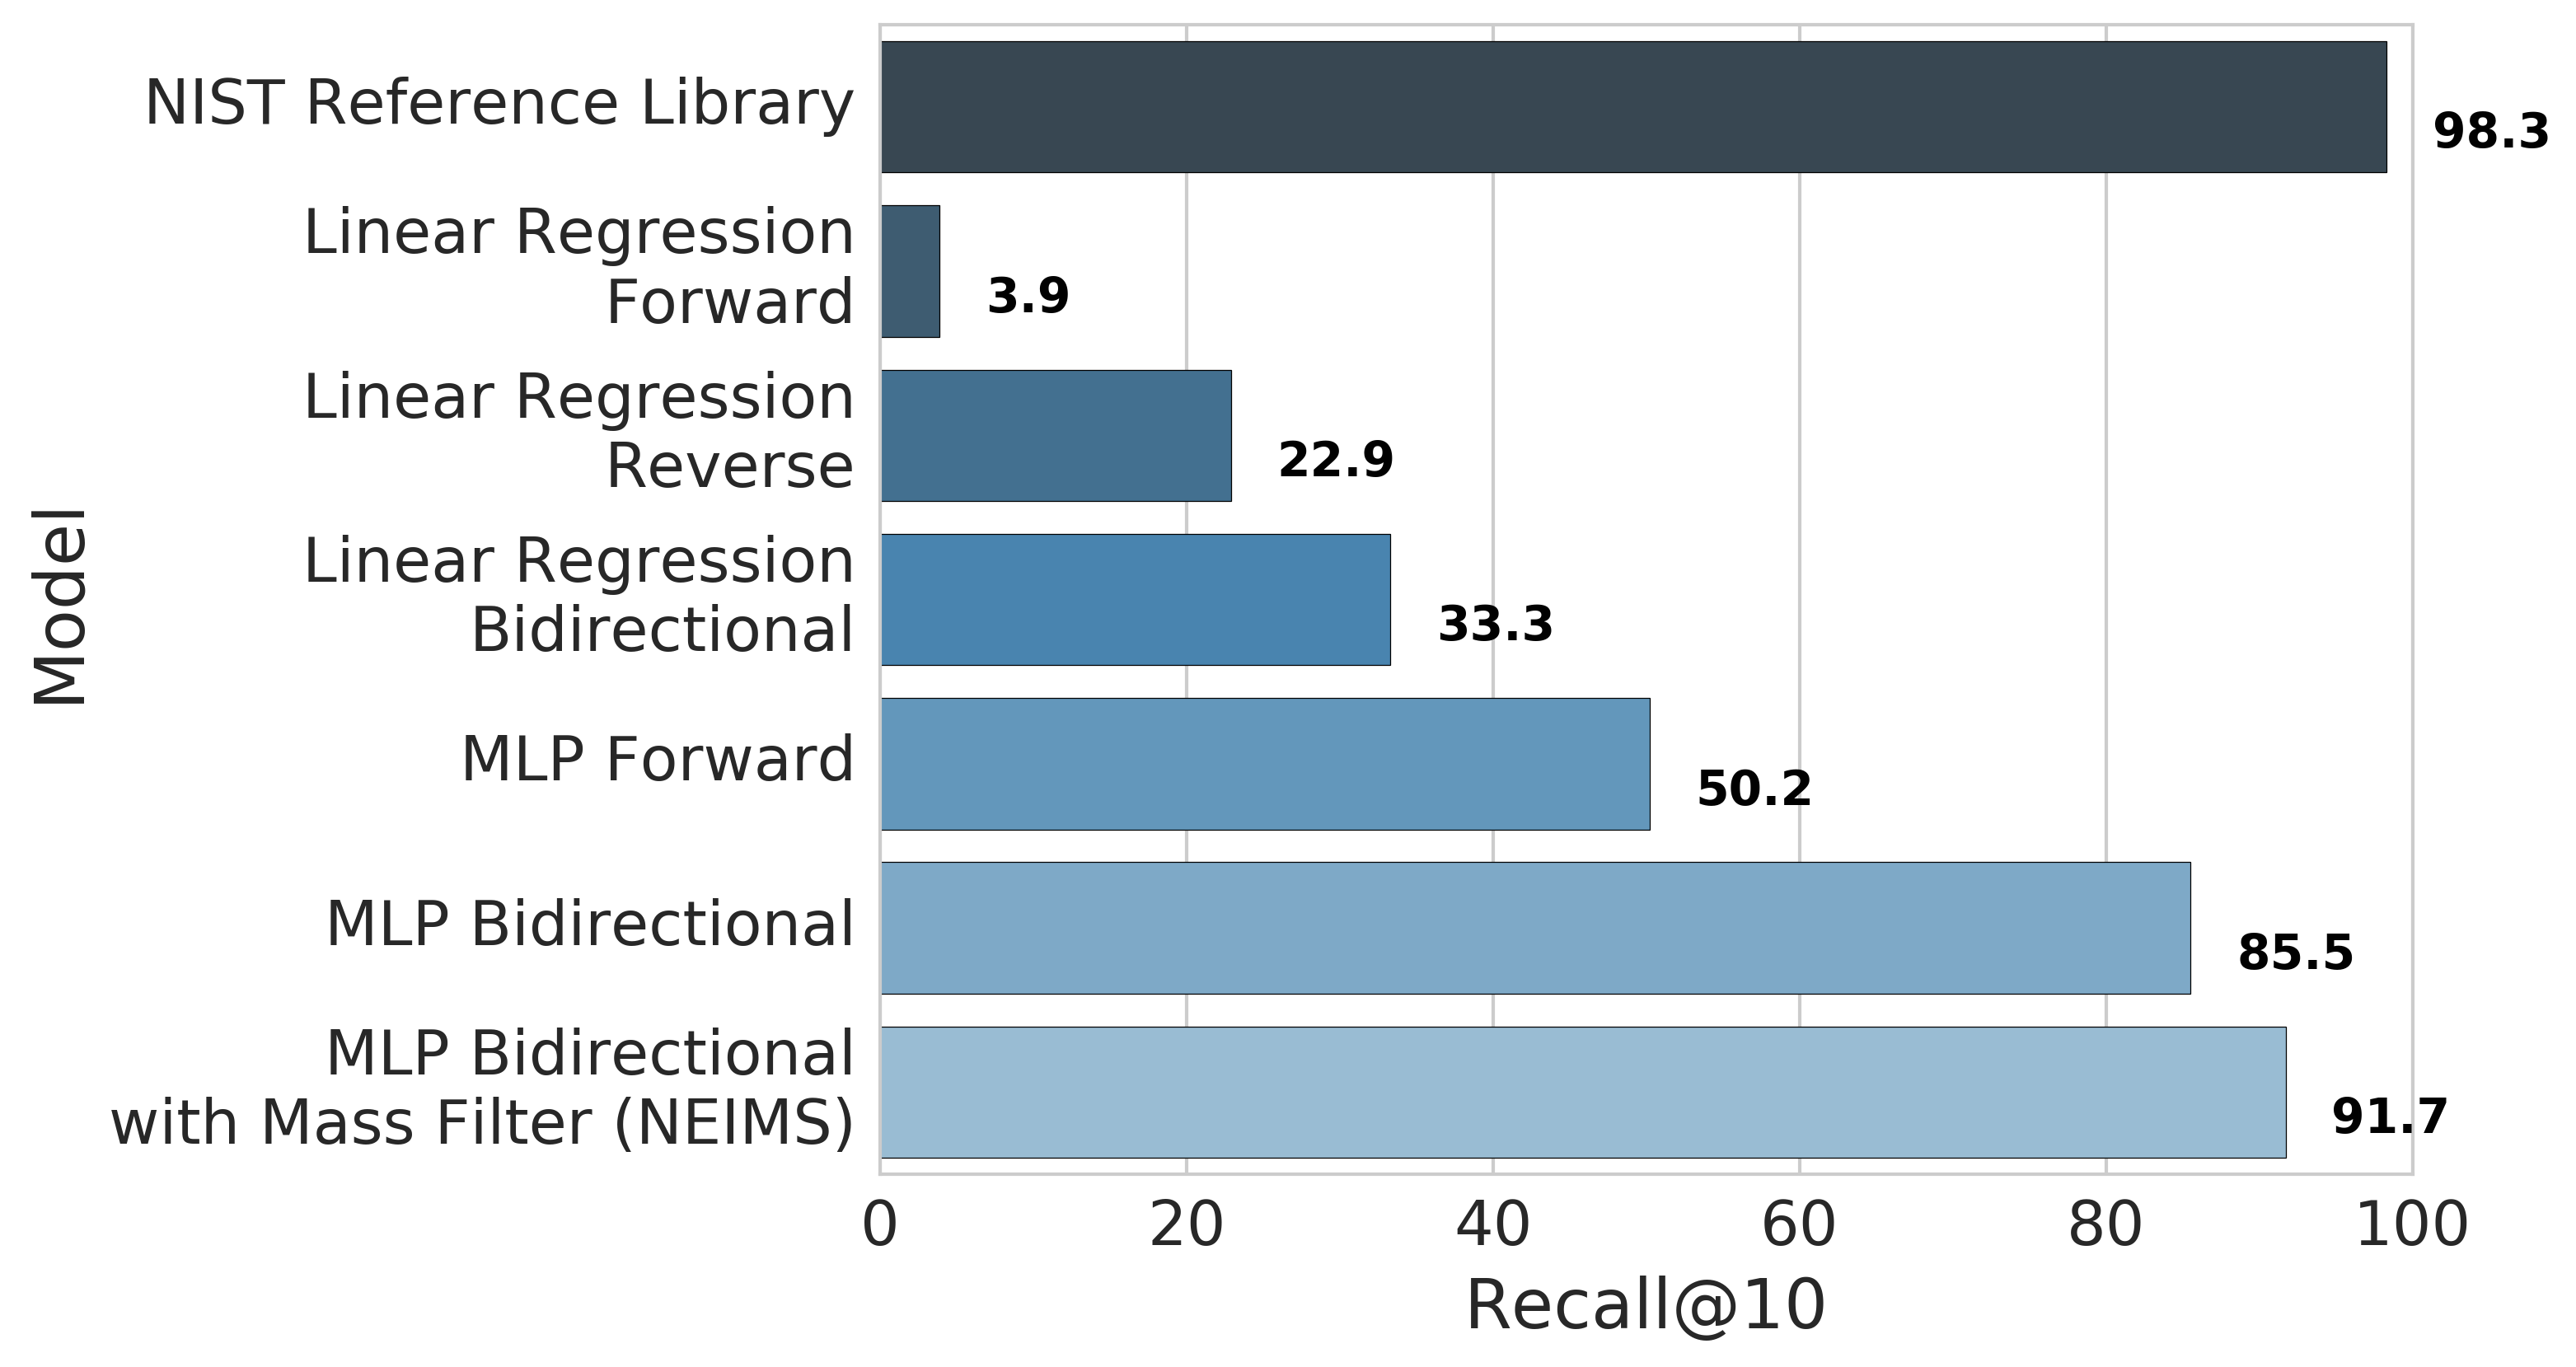
\includegraphics[width=\linewidth]{./all_models_w_massfilter.png}
        \caption[Library Matching Results]{Library matching performance on different models}
    \end{subfigure}
    \begin{subfigure}[b]{0.42\linewidth}
        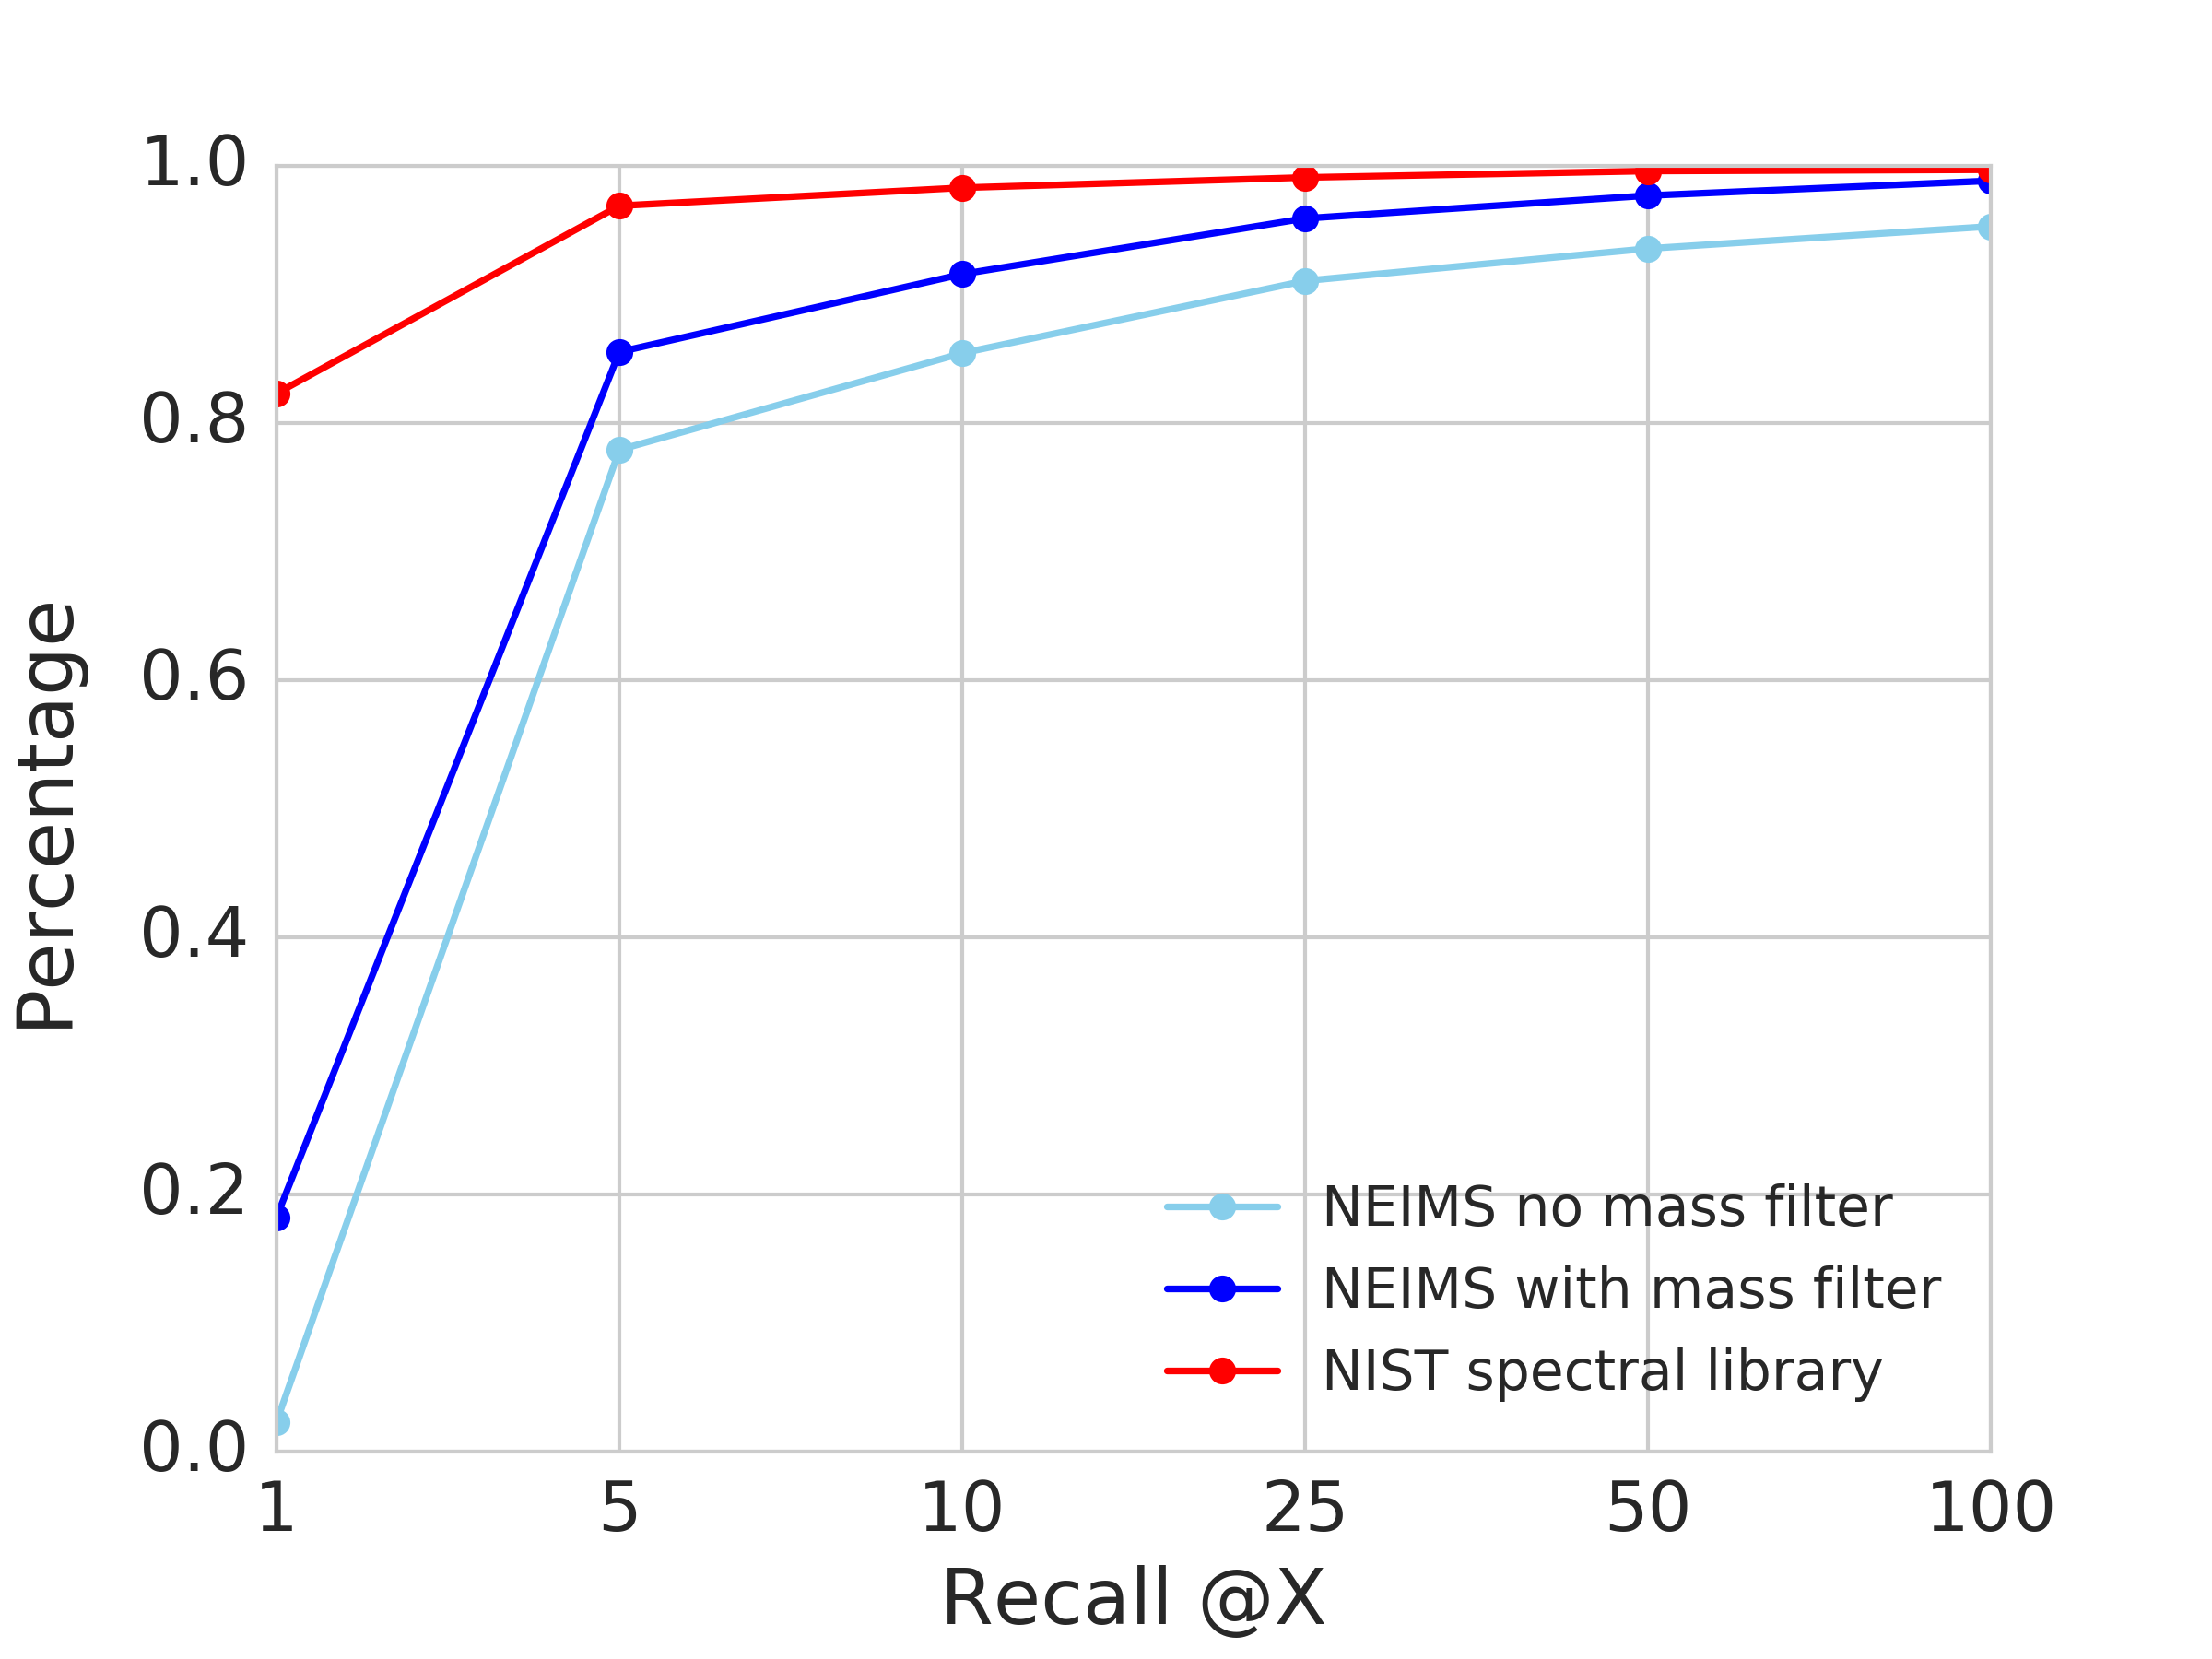
\includegraphics[width=\linewidth]{./recall_at_X.png}
        \caption[Recall@X Results for Different models]{Recall Results at various levels}
    \end{subfigure}
    \caption{Performance of different model architectures.}
    \label{fig:main_results_and_recall_results}
\end{figure}

We first examine the effects of our various modeling decisions on performance. Figure \ref{fig:main_results_and_recall_results}a compares the performance of forward, reverse, and bidirectional versions of the linear regression and MLP models on the library matching task. For bidirectional prediction in the linear regression model, the forward and reverse predictions are simply averaged together, rather than applying the gate described in \eqref{eq:sigmoid_gate}.

The top row of Figure \ref{fig:main_results_and_recall_results}a shows that it is not possible to achieve perfect recall accuracy on the library matching task even when using the full NIST main library as the reference library, without any model-predicted spectra. Observing Figure \ref{fig:main_results_and_recall_results}b we see that using the NIST main library as the reference library, we have 86\% recall@1 accuracy, and 98.3\% recall@10 accuracy. This serves as a practical upper bound on achievable library matching accuracy and reflects the experimental inconsistencies between between the main library spectra and replicates spectra~\cite{stein2012MassLibReview}.

The forward prediction mode for both the linear regression model and the multilayer perceptron (MLP) has poor performance. The linear regression model is improved by ~20\% when switching to using  reverse mode prediction. Using  bidirectional prediction mode improves  recall@10 accuracy by 30\% for both the linear regression and the multilayer perceptron model. This finding suggests that the bidirectional prediction mode is more effective at capturing the fragmentation events than the forward-only model.

Figure \ref{fig:MLP_improvement_spectra} shows the improvement in spectral prediction for pentachlorobenzene using the bidirectional MLP model. Note that the bidirectional model on the right more accurately models intensities at larger \textit{m/z}. The intensity peaks for larger \textit{m/z} are critical for determining the identity of a molecule, and are more heavily weighted in Eq.~\eqref{eq:stein-similarity}.

NEIMS achieves 91.7\% recall@10 after applying a mass filter. The mass filter was set to a tolerance of 5 Daltons of the query molecule's mass; this reduces the size of the library to a median of 6,696 spectra for each query molecule. In practice, this tolerance window could be set to a larger window, depending on the uncertainty of the information about the molecular mass of the ion.
For the rest of this report, we will refer to the bi-directional multi-layer perceptron model with mass filtering of 5 Daltons as the default settings for NEIMS.

From Figure \ref{fig:main_results_and_recall_results}b we see that while NEIMS has decent performance for recall levels of 10 and above compared to the NIST spectral library, it has considerably worse performance for recall values of 1 and 5. This result is unsurprising given that the hyperparmaters of the model were trained to maximize performance on recall@10.
If recall@1 was instead selected to tune the hyperparameters, the performance accuracy on recall@1 would improve.
%however this model becomes much more difficult to train due to the small amount of signal during the initial training of the model.

\subsection{Comparison to previously reported models}
\label{sec:NIST14-results}

We next compared our model's performance directly to the performance of the CFM-EI model~\cite{allen2016computational}. The setup of Allen et al. differs from our current setup in a few ways. First, they evaluate their model on the NIST '14 spectral library. Second, for the library matching task, their augmented reference library contains only spectra predicted by their model, and none from the original NIST collection. Third, the cosine similarity metric Eq. \eqref{eq:stein-similarity} used for evaluation in library matching in CFM-EI uses a different weighting scheme. In their analysis, the cosine similarity is weighted by $m_k^{0.5}$ instead of $m_k$ in order to de-emphasize the larger peaks in the mass spectrum, as they ran their experiments on other datasets with a higher proportion of larger molecules~\cite{allen2016computational}.

To compare the performance of NEIMS to that of CFM-EI, we match their setup identically. We retrain our NEIMS model on the NIST 14 dataset, and evaluate the performance using the NIST 14 replicates as the query set. For library matching, we incorporate only predicted spectra into our augmented library, and using the same modified similarity metric.

\begin{table}[t]
    \centering
    \begin{tabular}{cccc}
        Model & Recall@1 & Recall@10 (\%) &  Average run time (ms) \\
        \hline
        NIST '14 Reference Library & 77 & 99* & -- \\
        CFM-EI & 42.6 & 89* &  300,000 \\
        NEIMS & 54.3 & 92.7 &  0.47
    \end{tabular}
    \caption{Performance on Library matching task for NIST 17. * indicates that values were estimated from  Figure 4 of Allen et al.~\cite{allen2016computational}}
    \label{tab:NIST14_results}
\end{table}

The library matching performance for CFM-EI and NEIMS are compared against the NIST14 library for library matching performance are reported in Table \ref{tab:NIST14_results}. NEIMS performs slightly better than CFM-EI on the library matching task. More importantly, NEIMS is able to make spectral predictions orders of magnitude faster than CFM-EI.  With NEIMS, it would be possible to generate spectra for 1 million molecules in 90 min on a CPU, with potential for considerable speedup with using GPU.


\subsection{Distances between predicted and ground truth spectra}

\begin{figure}[t]
    \centering
    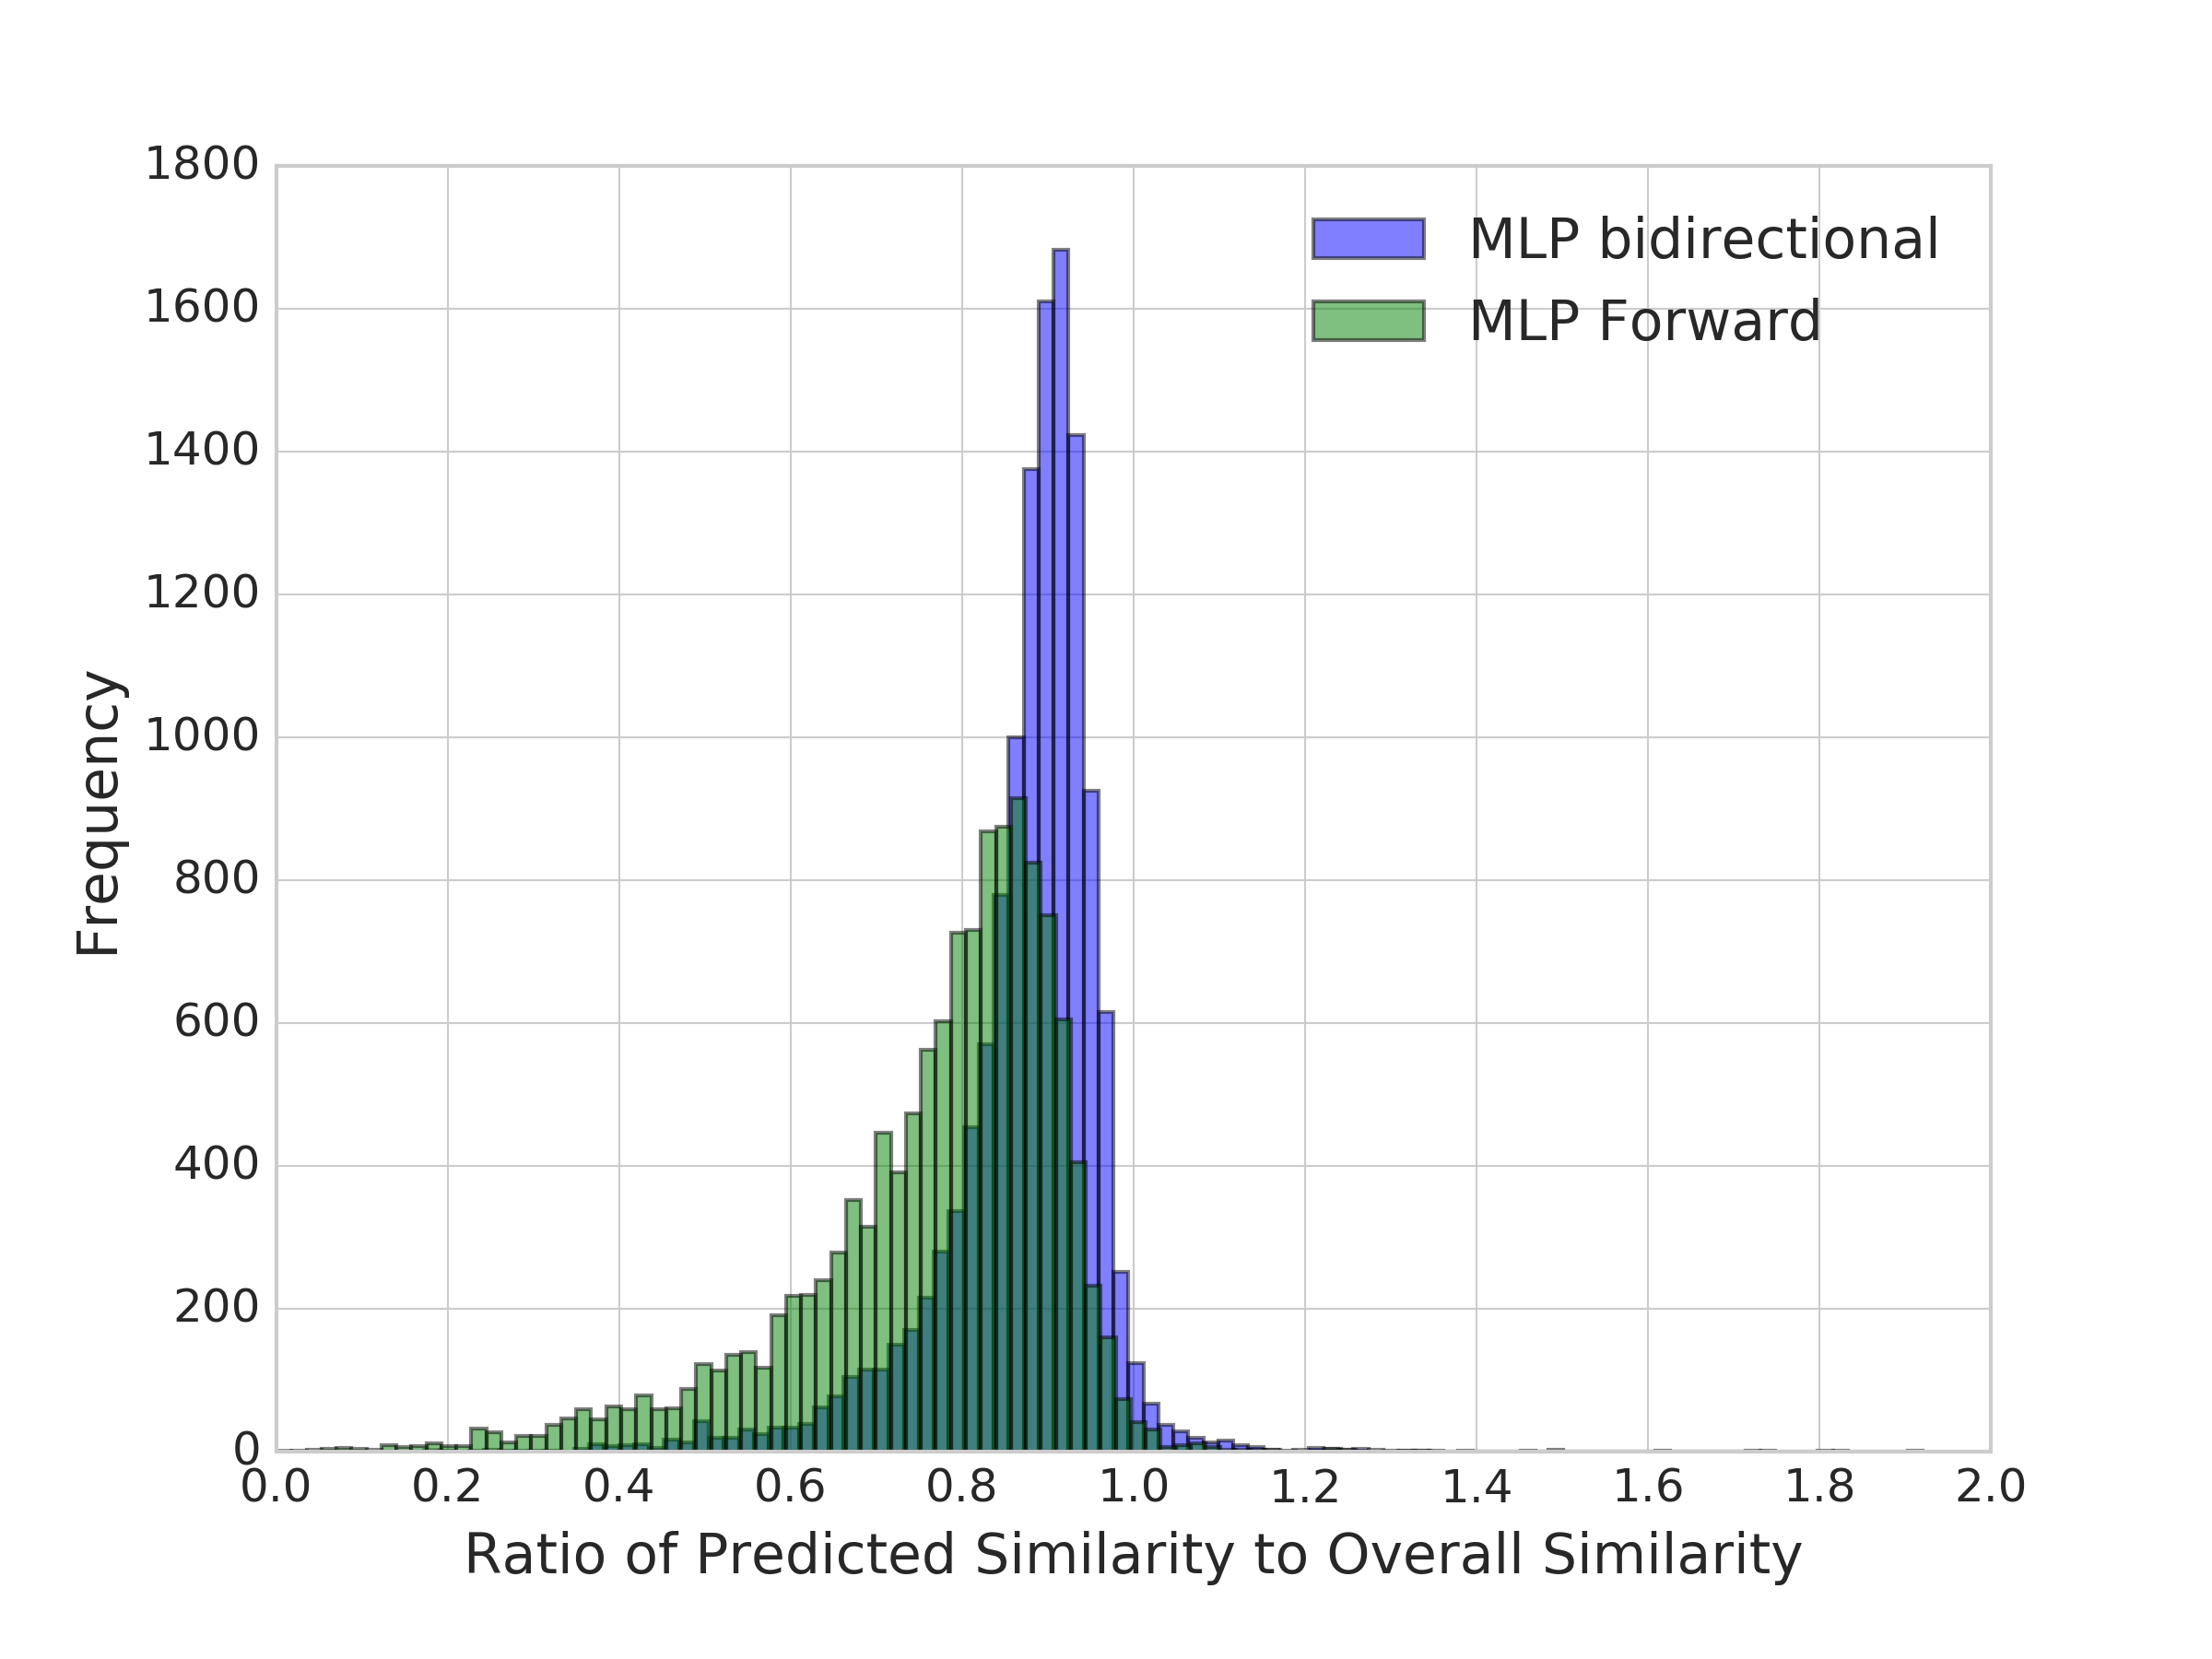
\includegraphics[scale=0.4]{./predicted_similarity_overall_similarity_ratio.png}
        \caption[Similarity Analysis of NEIMS predicted spectra to spectra self-similarity]{Comparing the similiarity between the predicted spectrum and the ground truth spectrum to the overall similarity between spectra for the same molecule. }
    \label{fig:similarity_analysis}
\end{figure}

So far, we have evaluated the quality of the NEIMS predictions indirectly, by way of how they affect library matching with an augmented library. Next, we assess the prediction accuracy directly, by measuring the similarity (Eq.~\ref{eq:stein-similarity}) between spectra in the NIST main library and the model's predictions. We refer to this similarity as the \textit{predicted similarity}.

There is inherent noise in mass spectra due to stochasticity of the underlying physical process and also to experimental inconsistencies~\cite{stein2012MassLibReview}. The NIST replicates library provides multiple spectra for each molecule, and we can use these sets of spectra to characterize the scale of this noise for each molecule. Specifically, we define the inherent noise for a given molecule as the average pairwise similarity between all corresponding spectra, both in the NIST main library and the NIST replicates library, and refer to this as the \textit{overall similarity}.

For each molecule, we compute the ratio of the predicted similarity to overall similarity as a normalized metric for the quality of our predictions. A ratio of 1.0 would suggest that there are is limited available headroom for improvements using machine learning, since the model's errors are comparable to the variability in the data.

Figure \ref{fig:similarity_analysis} shows the improvement in this ratio for the MLP bidirectional model over the MLP forward model, confirming that the bidirectional model has better spectral prediction performance. For the MLP bidirectional model, roughly half of the molecules have a predicted similarity to overall similarity ratio that is greater than 0.9, indicating that there is potential for further improvement to the model. Some of these molecules have ratios that are greater than 1, which is possible if there is more variation between the spectra (i.e. a lower overall similarity) than between the predicted spectrum and the main library spectrum (i.e. predicted similarity).

\section{Conclusion}

We demonstrate that NEIMS achieves high library matching performance on an augmented spectral library containing predictions for molecules in the query set.
The performance of NEIMS is also slightly better than existing machine learning models for predicting EI-MS spectra, with significant boost in speed of prediction.

The high performance in library matching is attributable to the bidirectional prediction mode. The reverse mode in particular allows the model to more accurately to predict intensities for larger fragments which result from the loss of small neutral subgroups. We observe that the improvement in the library matching task also corresponds with improvement in the similarity of the predicted spectra to the ground truth spectra.

Several adjustments could be made to further improve NEIMS. For example, NEIMS currently does not have a method to model intensity peaks corresponding to isotopes in ion fragments. If we were to train on spectral data with greater precision in the peaks locations, we might be able to learn the exact identities of the atoms based on the decimal values of the \textit{m/z} peak locations.

Mass filtering improved the performance of NEIMS by 6\%. This suggests that for experimental setups where it is possible to know the molecular mass of the sample with some accuracy, it is possible to improve the accuracy of matching on the augmented spectral library. It would also be interesting to explore other settings for mass filtering, such as filtering out spectra which have a molecular mass that is much smaller than the position of the largest \textit{m/z} peak.

Different molecular representations could also be tested. The predictions made from ECFP are limited by the descriptiveness of the fingerprint~\cite{rdkit_blogpost_collide_bits}. In particular, the overlap in representation for different molecular features represents a huge limitation to the representation of the molecule. Additionally, ECFPs are not equipped to represent molecules with multiple stereocenters, which will have different spectra. It would also be interesting to explore whether a bond-based molecular fingerprint representation \cite{kearnes2016molecular} or other graph-based molecular representations~\cite{duvenaud_convolutional_2015, gilmer_2017_mpnn} may improve performance.

Combining NEIMS with transfer learning methods could allow for spectral prediction specific to individual spectrometry machines. A library of such machine-specific spectra would improve matching~\cite{stein2012MassLibReview}.

The lightweight framework of NEIMS makes it possible to rapidly generate spectral predictions for large numbers of molecular candidates. This collection of predicted spectra can then be used directly in mass spectrometry software to expand the coverage of molecules which can be identified by mass spectrometry. Because the requirements of NEIMS has limited dependence to EI mass spectrometry, it likely that some of the principles used here could be extended to other types of mass spectrometry.


\section{Acknowledgments}
We thank Stephen Stein for fruitful discussions about mass spectrometry and for providing helpful feedback on this manuscript. We thank Laura Castellanos for her insights about mass spectrometry. We thank Steven Kearnes for his helpful comments, and Lucy Colwell and Michael Brenner for their helpful conversations.
